
\documentclass[14pt]{memoir}


% Lorem Ipsum Text
\usepackage{lipsum}

% Section and Figure Numbering
\renewcommand\thesection{\arabic{section}}
\usepackage{chngcntr}
\counterwithout{figure}{chapter}
\counterwithout{table}{chapter}

% Referencing Commands
\newcommand{\refsec}[1]{\hyperref[sec:#1]{Section~\ref{sec:#1}}}
\newcommand{\reffig}[1]{\hyperref[fig:#1]{Figure~\ref{fig:#1}}}
\newcommand{\reftab}[1]{\hyperref[tab:#1]{Table~\ref{tab:#1}}}

%TiKz
\usepackage{tikz}
\usetikzlibrary{arrows}
\usetikzlibrary{shapes}

%SidewaysFigure
\usepackage{rotating}

% CMU sans serif font.
\usepackage[T1]{fontenc}
\renewcommand*\familydefault{\sfdefault}

% Hyperlinks
\usepackage{hyperref}
\hypersetup{
    colorlinks=true,       % false: boxed links; true: colored links
    linkcolor=black,          % color of internal links (change box color with linkbordercolor)
    citecolor=black,        % color of links to bibliography
    filecolor=blue,      % color of file links
    urlcolor=blue           % color of external links
}

% APA 6 citation and bibliography style % Note: Must be loaded after hyperref
\usepackage{apacite} 

% Abbreviations
\usepackage{glossaries}
\makeglossaries

\newacronym{pisa}{PISA}{Programme for International Student Assessment}
\newacronym{oecd}{OECD}{Organisation for Economic Co-operation and Development}
\newacronym{stem}{STEM}{Science, Technology, Engineering and Mathematics}
\newacronym{fmri}{fMRI}{functional magnetic resonance imaging}
\newacronym{naplan}{NAPLAN}{National Assessment Program --- Literacy and Numeracy}
\newacronym{mars}{MARS}{Maths Anxiety Rating Scale}
\newacronym{mas-r}{MAS-R}{Maths Anxiety Scale --- Revised}
\newacronym{ptsd}{PTSD}{Post-Traumatic Stress Disorder}



\title{A Multifaceted Approach to Maths Anxiety}
\author{Lyron Winderbaum}



\begin{document}



\maketitle



\begin{abstract}

\lipsum[1-2]

\end{abstract}
% 100-150 words


\glsresetall
\section{Literature Review}

\subsection*{Prevalence}

Maths anxiety is hugely prevalent, and consequently the literature describing research around it is extensive. The \citeA{PISA2013} 2012 \gls{pisa} report states that across \gls{oecd} countries, over 30\% of 15 year old students ``get very nervous doing mathematics problems'', and over 60\% of students ``worry about getting poor grades in mathematics''. 

\subsection*{Why is Maths Anxiety Important?}

As teachers our foremost concern should be for the wellbeing of our students. It has been shown that students with a high level of maths anxiety often literally experience the anticipation of a maths task as visceral pain \cite{Lyons2012pain}. This helps to emphasise the clear and overwhelming moral imperative (and ethical duty of care) on us to do everything in our power to protect students in our care from maths anxiety.

Even if the wellbeing issue was not enough, there is also a clear maths anxiety-performance connection, and a complex web of stakeholders surrounding a students academic success in maths. One example of this is highlighted by \citeA{Foley2017} who juxtaposes the internationally rising demand for \gls{stem} professionals with the negative correlation between maths anxiety and performance shown in the 2012 \gls{pisa} \cite{PISA2013} report to highlight the relevance of addressing maths anxiety in filling this demand. This relationship between maths anxiety and maths-qualified professionals in the workforce is supported throughout the literature: when a student has low self-concept (correlated with high maths anxiety), they will tend not to enroll in maths beyond the minimum requirements for graduation \cite{Ashcraft2007book}, and students affect towards maths can predict their university major \cite{LeFevre1992}. Beyond this example, the list of stakeholders in a students academic success in maths goes on and on: parents; the student's themselves; schools (which are often funded based on the results of standardised testing such as \gls{naplan}), and teachers amongst them. 

Students success in maths, as well as their wellbeing, is important to many parties for many reasons. The one thing all the stakeholders agree on is that addressing maths anxiety is important, what nobody can agree on is exactly what maths anxiety is, how to measure it, and how to intervene and address it.



\subsection*{Frameworks for Understanding the Maths Anxiety-Performance Link}.

Due to the importance of the maths anxiety-performance link, the bulk of the literature is focused on it. Only a few studies focus on maths anxiety itself (primarily \gls{fmri} studies such as those of  \citeA{Young2012} or \citeA{Lyons2012pain}). There are good reasons for focusing on the maths anxiety-performance link rather than maths anxiety in isolation, as discussed above. In terms of understanding this link however, there seem to be two distinct theories being pursued amongst the academy and I will adopt the terminology of \citeA{Ramirez2018} to describe them: the ``Disruption Account'' and the ``Reduced Competency Account''. \citeA{Ramirez2018} go on to make a convincing argument that although these two theories might seem to compete, they are not actually mutually exclusive and instead quite compatible with each other. \citeA{Ramirez2018} suggests a third ``Interpretation Account'' which encapsulates observations made by both lines of research, see \reffig{ramirez}. This seems to be a fairly new idea, and one we will aim to test in this study. 

\begin{center}
\begin{figure}
\begin{center}
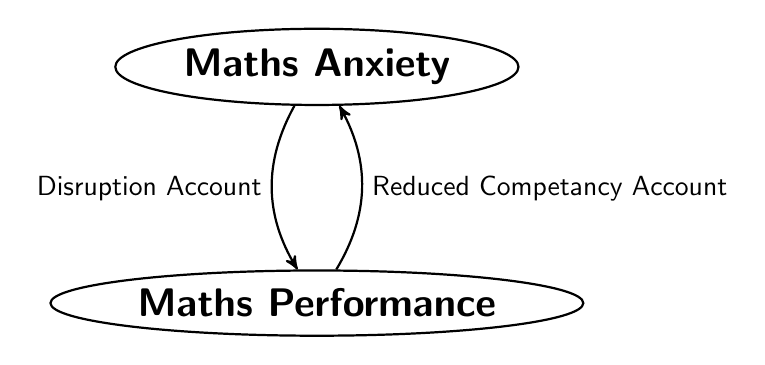
\begin{tikzpicture}[->,>=stealth',auto,node distance=3cm,thick,main node/.style={ellipse,draw,font=\sffamily\Large\bfseries}]
  	\node[main node] (a) {Maths Anxiety};
 	\node[main node] (b) [below of=a] {Maths Performance};

	\path	(a) edge[bend right] node [left] {Disruption Account} (b)
		(b) edge[bend right] node [right] {Reduced Competancy Account} (a);
\end{tikzpicture}
\end{center}
\caption{The Interpretation Account of Ramirez et al. (2018) for the maths anxiety-performance link showing how the Disruption Account and the Reduced Competency Account can be compatible.
\label{fig:ramirez}}
\end{figure}
\end{center}

First, a little more detail on the existing theories. The ``Disruption Account'' is currently considered as the dominant theory, seemingly spearheaded by the work of Ashcraft et al. and is based on a body of work centered around the concept of working memory \cite{Ashcraft2001, Ashcraft2007}. Specifically, the thought is that maths anxiety takes up students working memory, which prevents them from using that working memory to complete maths tasks and hence impacts performance. The ``Reduced Competency Account'', which seems to be less popular in recent times, claims that lower ability in maths leads to negative experiences associated to maths, and that these negative experiences cause maths anxiety to develop. There is also a significant body of work to support this hypothesis, including the meta-analysis of \citeA{Hembree1990} discussed above and more recent follow-up work such as the large longitudinal study of \citeA{Ma2004} which found that although past maths anxiety was correlated with future maths performance it was a small effect, while past maths performance had a strong effect on future maths anxiety.



\subsection*{Complexities in Finding Effective Interventions}

These theoretical views are of course broad oversimplifications of what is an incredibly complex and interconnected topic. They also imply very different approaches for intervention. The ``Reduced Competency Account'' would imply interventions to boost maths performance and hence allow students to experience success in math should also help to reduce maths anxiety. The results of  \citeA{Supekar2015} seem to support this hypothesis as when students are given an intensive 8-week tutoring program to boost their maths skills, this is associated to a reduction in maths anxiety. The earlier work by \citeA{Faust1996} further supports this by demonstrating an anxiety-complexity effect in which low and high maths anxiety groups performed similarly on low complexity problems, but in high complexity problems the high anxiety groups performance was impacted. On the other hand, \citeA{Jansen2013} showed that it is not neccessarily that simple, by showing that when students experience more success they attempt more problems and perform better. However their improved performance is almost completely predicted by the number of problems they attempted, not their experience of success, and their level of maths anxiety was not affected in a significant way. Which raises an important moral question: if we have interventions that improve students performance, but not their maths anxiety
	
On the other side of attempted interventions are those in line with the ``Disruption Account'', in which the maths anxiety itself is addressed in the hopes that will free up extra working memory and hence boost students performance. One fairly direct and successful attempt at this is that of \citeA{Park2014}, in which they used expressive writing exercises to help guide students self-perceived narratives about their maths experiences and thereby reduce their maths anxiety. Notably the approach of \citeA{Park2014} is in line with successful treatments for clinical anxiety disorders (see \citeA{McNally2007, Becker2007,Foa2005}). Another approach that has shown success in this vein does not attempt to directly reduce the anxiety experienced, but rather reappraise it's symptoms \cite{Jamieson2016}. This is another technique from clinical psycology in which stress is reconceptualised as a coping tool, an evolutionary method for heightening performance in response to a challenge to be overcome, instead of a symptom of exposure to something to be feared and avoided. This change in the perspective students have of stress is also very much in line with the ``Interpretation Account'' of \citeA{Ramirez2018}.

The work of \citeA{Wang2015} showed the role that intrinsic motivation has mediating the relationship between maths anxiety and performance, and suggested the importance of a mindset centred on viewing the process of learning maths as one of ``productive struggle''. This reconceptualisation to a `productive struggle' model is supported by other literature as well, \citeA{Lin-Siegler2016} exposes students in a classroom to struggles experienced by famous scientists in order to help normalise the concept of productive struggle, and \citeA{Hiebert2007} discuss the importance of this same concept in a maths context.

One of the implications of the ``Interpretation Account''  not predicted by either of the two major theories out there right now is that after an intervention the other, untreated, direction will re-establish the cycle shown in \reffig{ramirez} and that in the longterm the intervention will be relatively ineffective even if it has shortterm results. Several authors have mentioned the need for more longitudinal research surrounding interventions for maths anxiety \cite{Pellicioni2016,Chang2016}. Notably the there is the study of \citeA{Ma2004} mentioned above, but otherwise there are very few such longitudinal studies, and those that exist have shown mixed results. My hypothesis is that with a multi-faceted approach targetted multiple causation pathways interlinking maths anxiety and performance, the entire cycle can be disrupted and result in a more positive long-term effects than individual interventions alone.



%\subsection*{Maths Anxiety as Distinct from General Anxiety}
%
%The existence of maths anxiety as ``emotional disturbances in the presence of mathematics'' has been noted as early as the 1950's, \citeA{Dreger1957} even postulated that what he tentatively designated ``Number Anxiety'' and later became to be known as Maths Anxiety could be a distinct syndrome from general anxiety. Later the landmark meta-study of \citeA{Hembree1990} supported this hypothesis, showing a correlation of only $0.38$ between maths anxiety and general anxiety. In more recent times, this hypothesis has also been confirmed by \citeA{Young2012} using \gls{fmri} to show that the brain activity in a person experiencing maths anxiety is measurably distinct from that in a person suffering general anxiety. These later studies, as well as the the work of \citeA{Kazelskis2000} and more, have also delineated maths anxiety from test anxiety, and these different anxieties exisitng as meaningfully distinct constructs is now quite well accepted. For more on the history of maths anxiety, \citeA{Pellicioni2016} offers a more detailed review.



\section{Research Proposal}

I propose a multifaceted intervention in which multiple links in the cycle (see \reffig{ramirez}) are attacked simultaneously to disrupt the maths anxiety-performance link. I hypothesise that this approach will result in a more longlived effect on both students wellbein (anxiety) and maths performance. The four facets of the proposed intervention are:
\begin{itemize}
	\item An intensive tutoring program to boost students math abilities, along the same lines as that of \citeA{Supekar2015}.
	\item Coaching around reappraisal of physiological signs of stress (increased heart rate, sweaty palms, etc.) such as that of \citeA{Jamieson2016} to interpret these signs as an evolutionary trait that increases fitness and performance in response to a challenge, instead of interpreting them as signs of danger to run from and avoid.
	\item Guided expressive writing, such as the approach of \citeA{Park2014}, inline with existing exposure therapy approaches from clinical psychology.
	\item Coaching around perceiving the process of learning maths as one of ``productive struggle'' \cite{Hiebert2007}.
\end{itemize}



\subsection*{Instruments for Measuring Maths Anxiety}

In order to track the effectiveness of these interventions, we will be collating assessment results as a measure of performance, but will also want to measure maths anxiety and maths affect/ self-concept. 

Significant work has been done over the years to develop psychometrics to measure maths anxiety, almost exclusively consisting of self-reporting surveys (with the exception of some more modern \gls{fmri} work, such as that of \citeA{Lyons2012}). One of the earliest instruments for measuring maths anxiety was the \gls{mars} 98-item 5-point Likert scale of \citeA{Richardson1972}. Since then, many different groups have split off and created various revised versions of a number of offshoots of this original idea, but all rely on a self-reporting survey. One of the more recently developed scales is the \gls{mas-r} of \citeA{Bai2009}, which has been shown to be remarkably self consistent by incorporating both positive and negative affect items \cite{Bai2011}, and due to this property as well as the fact that it is short and easy to imlement is the one we will use to measure maths anxiety.

\citeA{Jansen2013} modified the Perceived Competence Scale for Children \cite{Harter1982} to measure ``Math Competance''. Although this extended scale doesn't seem to have comparative consistency studies done on it, the internal checks \citeA{Jansen2013} were quite rigorous and so we will use their instrument to measure maths self-concept, although in English.



\subsection*{Timeline}

Each intervention will be introduced sequentially, with at least a 3-week gap between them to allow for a multivariate time-varying autoregressive model to be fitted in order to investigate individual effects. 

 \begin{sidewaysfigure}
 \includegraphics[scale=0.7]{Gantt_Chart.PNG}
\caption{Gantt Chart \label{fig:gantt}}
\end{sidewaysfigure}

\begin{table}[p]
\begin{center}
\includegraphics[scale=1.2]{Budget.PNG}
\end{center}
\caption{Budget \label{tab:budget}}
\end{table}

The proposed timeline for 2020 is shown in \reffig{gantt} in which the bulk of the study will be conducted, but to summarise:
\begin{itemize}
	\item 2019: Assessment instruments and instruction programs will be developed and fine-tuned.
	\item Teacher coaching sessions will begin immediate commencing 2020.
	\item Term 1 Week 4: Intensive tutoring program begins.
	\item Term 1 Week 7: Guest Speaker on productive struggle, and teachers will start implmenting productive struggle program. 
	\item Term 2 Week 4: Guest speaker will return, refresh productive struggle talk and give reappraisal talk. Teachers will begin reappraisal program while continuing to use examples of productive struggle.
	\item Term 2 Week 7: Expressive writing excercise.
	\item Terms 3 and 4: productive struggle, reappraisal, and expressive writing excercises are continued by teachers, tutoring program ends in term 3.
	\item 2021: Students will return to ordinary classes.
\end{itemize}

There will be a number of streams of ongoing primary data collection throughout:
\begin{itemize}
 	\item  During school holidays there will be teacher debrefiing sessions in which the teachers will be asked to provide feedback on their perspectives on the effects of the interventions.
 	\item Academic results of students will be collated for an entire three year 2019-2021 period.
 	\item Students will complete self-surveys on both maths anxiety, and maths self-concept the year prior, during, and the year after the interventions. These will occur before and after the introduction of each facet of the intervention, allowing for multivariate interaction effects to be modelled.
 	\item The expressive writing tasks will yield written work from each student describing their narative view of their journey learning maths, which can also be used to assess their self-concept/ efficacy in a deeper way.
\end{itemize}



\subsection*{Budget}

This research is predicated on collaborating with a school and the maths faculty therein, and the leadership team at the school being on board. The budget proposed above (see \reftab{budget}) presupposes $30$ student participants either in one class or split accross two classes, $1-2$ teacher participants, and for the entire study to be performed over the three year period 2019-2021. Should additional funding be made available, it would be possible to extend the study to include a larger sample of students and teachers, and to continue monitoring the students into 2022-2023, which would offer very valuble additional data on the longer term effects of the interventions.



\section{Ethics Issues}

Some key ethical considerations include:
\begin{itemize}
	\item All stakeholders (Teacher and student participants as well as parents and school leadership) will be given the full experimental details prior to commencement of the study. 
	\item All published results will be fully anonymised.
	\item Students and parents will be made aware they have the option to opt-out at any time. Any student that wishes to be withdrawn during the study will be moved to a class not participating in the study. Withdrawn data will be ommitted from all analyses, the only remaining trace a note of the total number of students that were withdrawn.
	\item Teachers will have complete autonomy running their classes, and will have the right to stop the study at any time should they beleive it to be causing any harm (emotional, or academic) to the students. This judgement will be at the discretion of the teachers involved in consultation with the leadership team.
	\item All content addressing anxiety and other sensitive topics will include appropriate trigger warnings, a school councillor and a ``cooling off space'' will be available at all times should a student find themselves in distress.
\end{itemize}


\section{Executive Summary}



\printglossaries

\glsresetall
\bibliographystyle{apacite}
\bibliography{citations} 

\end{document}


